\section{Центр масс}
%TODO решение задачи про цепную линию
\begin{ex}
Тонкий однородный стержень длиной $l$ и массой $m$ привели в движение вдоль гладкой горизонтальной поверхности так, что он движется поступательно и одновременно вращается с угловой скоростью $\omega$ вокруг оси перпендикулярной стержню и проходящей через его центр. Найдите натяжение стержня в зависимости от расстояния $x$ до его центра.
\begin{ans}
$T(x) = m \omega^2 \left( l^2 - 4x^2 \right)/8l$
\end{ans}
\end{ex}

\begin{ex}
Двойная звезда состоит из двух звезд-компонентов массами $m_1$ и $m_2$, расстояние между которыми не меняется и остается равным $L$. Найдите период вращения двойной звезды.
\begin{ans}
$T = 2 \pi \sqrt{\frac{L^3}{G(m_1+m_2)}}$ 
\end{ans}
\end{ex}

\begin{ex}
(2009) Невесомый стержень длины $L$ с двумя шариками на концах с массами $m$ и $3m$ находится на гладкой горизонтальной поверхности. Шарику массой $m$ резко сообщают скорость $\vec v$ в направлении перпендикулярном стержню. Какова сила натяжения стержня? Как изменится ответ, если скорость $\vec v$ сообщить шарику массой $3m$? Какая часть энергии перейдет в кинетическую энергию вращательного движения в первом и во втором случаях?
\begin{ans}
В первом случае $T = 9mv^2 / 4l$, в кинетическую энергию вращения перейдет $3/4$ энергии
\end{ans}
\end{ex}

\begin{ex}
\hspace{0pt} \\
(1998) На гладкой горизонтальной плоскости лежат два одинаковых бруска массой $m$ каждый, связанные легкой пружиной жесткостью $k$. Первому бруску сообщают скорость $v_0$ в направлении от второго бруска. Опишите движение системы. Через какое время деформация пружины впервые достигнет максимального значения? 
\begin{center}
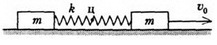
\includegraphics[width = 0.4 \textwidth]{051998CenterOfMassSpring.jpg}
\end{center}
\begin{ans}
$T = \frac{\pi}{2}\sqrt{\frac{m}{2k}}$
\end{ans}
\end{ex}

\begin{ex}
Шар массой $m$ налетает со скоростью $v$ на покоящийся шар массой $2m$. Найдите скорости обоих шаров после упругого центрального удара. 
\begin{ans}
$v_1 = v/3$, $v_2 = 2v/3$
\end{ans}
\end{ex}

\begin{ex}
Определите, какую часть своей кинетической энергии теряет частица массой $m_1$ при упругом лобовом столкновении 
с неподвижной частицей массой $m_2$. 
\begin{ans}
$4m_1m_2/(m_1+m_2)^2$
\end{ans}
\end{ex}

\begin{ex}
Известно, что при упругом нецентральном ударе двух одинаковых шаров, один из которых до удара покоился, угол разлета равен $90^{\circ}$. Докажите это утверждение.
\end{ex}

\begin{ex}
(2012) На абсолютно гладком столе лежит обруч массой $M$ и радиусом $R$. На обруче находится жук, масса которого $m$. Какие траектории будут описывать жук и центр обруча при движении жука по обручу?
\begin{ans}
Окружности радиусами $r_1 = mR/(m+M)$ и $r_2 = MR/(m+M)$
\end{ans}
\end{ex}

\begin{ex}
\hspace{0pt} \\
\begin{minipage}{.65\textwidth}
Клин массой $2m$ с углом наклона к горизонту $\alpha $ ($\cos~\alpha$~=~2/3) находится на гладкой горизонтальной поверхности стола. Через блок, укрепленный на вершине клина, перекинута легкая нить, связывающая грузы массами $m$ и $3m$. Груз массой $3m$ может скользить вдоль вертикальной направляющей АВ, закрепленной на клине. Этот груз вначале удерживают неподвижно на расстоянии $H$~=~27~см от стола, а затем отпускают. На какое расстояние сместится клин к моменту касания груза массой $3m$ стола? Массами блока и направляющей АВ пренебречь.
\end{minipage}
\begin{minipage}{.35\textwidth}
\centering
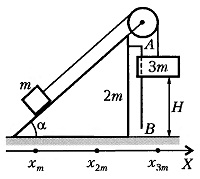
\includegraphics[width = 0.9 \textwidth]{0510CenterOfMassWedge.jpg}
\end{minipage}
\begin{ans}
$x = 3$ см
\end{ans}
\end{ex}

\section{Распределенная масса}

\begin{ex}
Струя воды сечением $S$ ударяется о стенку, расположенную перпендикулярно струе. Скорость воды в струе $v$, после удара вода теряет скорость и стекает по стенке. Какова сила давления воды на стенку? Плотность воды $\rho$.
\begin{ans}
$F = \rho S v^2$
\end{ans}
\end{ex}

\begin{ex}
Космический корабль массой $M$ движется в глубоком космосе. Для управления кораблем используется реактивный двигатель, который выбрасывает реактивную струю со скоростью $u$ относительно корабля, причем расход топлива в струе равен $\mu$ (расход топлива -- это масса топлива, выбрасываемая за единицу времени). Найдите ускорение корабля.
\begin{ans}
$\vec a = - \mu \vec u / M$
\end{ans}
\end{ex}

\begin{ex}
Тонкое веревочное кольцо массой $m$ и радиусом $R$ положили на гладкую горизонтальную поверхность и раскрутили до угловой скорости $\omega$. Найдите силу натяжения веревки.
\begin{ans}
$T = m\omega^2R/2 \pi$
\end{ans}
\end{ex}

\begin{ex}
Чтобы остановить движение большого судна при причаливании, с него на пристань бросают канат и насколько раз оборачивают вокруг тумбы. В результате, прикладывая небольшое усилие к свободному концу проскальзывающего каната можно остановить огромный пароход. Рассчитать, во сколько раз действующая на пароход со стороны каната сила превосходит приложенное к свободному концу каната усилие, если число оборотов равно $n$, коэффициент трения каната о тумбу $\mu$.
\begin{ans}
$e^{2\pi \mu n}$
\end{ans}
\end{ex}

\begin{ex}
\hspace{0pt} \\
\begin{minipage}{.65\textwidth}
(2011) Однородная цепочка длиной $L$ и массой $m$ подвешена на нити так, что другим концом она касается стола. Нить пережигают. Найти зависимость силы давления $F$ цепочки на стол от длины $x$ еще не упавшей части. Считать удар звеньев о стол неупругим.
\end{minipage}
\begin{minipage}{.35\textwidth}
\centering
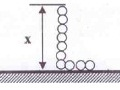
\includegraphics{0507DistributedMassChainAndTable.jpg}
\end{minipage}
\begin{ans}
$F = 3mg(1-x/l)$
\end{ans}
\end{ex}

\begin{ex}
\hspace{0pt} \\
\begin{minipage}{.65\textwidth}
Длинная тонкая цепочка перекинута через блок так, что ее правая часть свисает до пола, а левая лежит, свернувшись клубком, на уступе высотой $H$. Цепочку отпускают, и она приходит в движение. Найдите установившуюся скорость движения цепочки. Блок идеальный, цепочка неупругая.
\end{minipage}
\begin{minipage}{.35\textwidth}
\centering
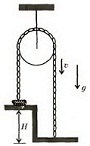
\includegraphics{0503DistributedMassChainAndPulley.jpg}
\end{minipage}
\begin{ans}
$v = \sqrt{gH}$
\end{ans}
\end{ex}

\begin{ex}
\hspace{0pt} \\
\begin{minipage}{.65\textwidth}
Веревку длиной $l$ и массой $m$ кладут на гладкое горизонтальное бревно радиусом $R$, причем вначале веревку удерживают за верхний конец, прикладывая горизонтальную силу $F$, а затем отпускают. Определите: 1) значение силы $F$; 2) ускорение веревки в первый момент.
\end{minipage}
\begin{minipage}{.35\textwidth}
\centering
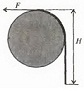
\includegraphics{0505DistributedMassRope.jpg}
\end{minipage}
\begin{ans}
$F = mgH/l$, $a = gH/l$
\end{ans}
\end{ex}

\begin{ex}
\hspace{0pt} \\
\begin{minipage}{.65\textwidth}
Цепочку массой $m$ и длиной $l$ подвесили за концы к потолку. При этом оказалось, что в местах закрепления цепочка образует углы $\alpha $ с вертикалью. Найдите расстояние $h$ от нижней точки цепочки до потолка.
\end{minipage}
\begin{minipage}{.35\textwidth}
\centering
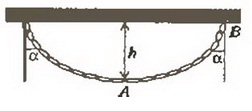
\includegraphics[width = 0.9 \textwidth]{0506DistributedMassChainAndCeiling.jpg}
\end{minipage}
\begin{ans}
$h = l(1 - \sin \alpha)/2 \cos \alpha$
\end{ans}
\end{ex}

\begin{ex}
Определите форму тяжелой нерастяжимой цепочки, подвешенной за концы на одной высоте, в однородном поле силы тяжести.
\begin{ans}
$y = a \cosh x/a$, $a = T/\rho g H$
\end{ans}
\end{ex}
